\subsection{General Strategy Overview}
This could also be an introductionary text which motivates the following subsections.

%%%%%%%%%%%%%%%%%%
\subsection[Agent Specific Strategies]{Agent Specific Strategies$^\dagger$}\label{alg:agentstrategies}
Because each of the five different agent types (or \emph{roles}) in the MAPC scenario --- Explorers, Repairers, Saboteurs, Sentinels and Inspectors --- have different capabilities in terms of the actions they can perform, they must each act according to role-specific strategies and tactics in order for the team to perform well.
This section will give a short overview of how different agent types behave differently from each other.
\begin{description}
    \item[Explorer] agents are the only ones who can perform the \texttt{probe} action.
        Vertices must be probed in order to learn their value, which is critical for zoning.
        Accordingly, an Explorer will spend most of his time seeking out, moving towards and finally probing vertices whose value is not yet known.
        Since there are 6 Explorers in a team, care must be taken to make sure that multiple Explorers do not move towards the same unprobed vertex, as this is generally a suboptimal usage of their time.

        In our implementation, we consider all vertices in the map to be \enquote{worthy} of being probed and thus to know their value.
        However, due to the way our team performs zoning (see~\autoref{alg:zon_finding}), we prioritise vertices in a specific way which we call \enquote{cluster probing}.
        Because our zone calculation algorithm (see~\autoref{alg:zon_calculation}) puts agents around a centre vertex in a circular manner and with a maximum distance of two edges away, and because we want the Explorers' probing to help us with quickly finding and establishing high-value zones, Explorers should avoid probing vertices in e.g.\ a straight line.
        Rather, an Explorer's probing pattern should mimic the circular shape of the zone calculation algorithm.
        Because of this, for probing we prioritise unprobed vertices first by distance, then by the number of edges they share with already probed vertices.
        The result is that Explorer movement is similar to a spiral pattern (provided the Explorer is not disturbed by e.g.\ nearby enemy agents).
        Explorer agents do not stop this probing pattern until they can no longer find any unprobed vertices.
    \item[Repairer] agents are the only agents who can perform the \texttt{repair} action for restoring health to disabled agents.
        Because the team loses out on possible points for every disabled agent in the team, to achieve a high score it is essential to quickly repair damaged agents.
        In our implementation, Repairers' actions are prioritised so that they will attempt to repair any disabled friendly agent in their visibility range, and it is the \enquote{job} of the disabled agents to find and move towards the closest friendly repairer.
        If a Repairer agent is aware of a friendly disabled agent outside of his visibility range, and the Repairer is currently not used for zoning, however, then the Repairer will also move towards the disabled agent.
    \item[Saboteur] agents are the only agents that can disable enemy agents using the \texttt{attack} action.
        In our implementation, a saboteur's role is very aggressively defined, and is prioritised thusly: if you see a non-disabled enemy, attack it; otherwise find and move towards an enemy you can attack.

        Throughout most of our development phase, Saboteur agents were the only agent type we would use the \texttt{buy} action for to extend their visibility range once for every Saboteur because we believed that this would give us an offensive edge against other teams.
        We decided to try out other buying strategies as well, however, by having our agents play matches against copies of themselves, except that the copies used different strategies for buying upgrades.
        Through this brief, empirical and rather informal testing period, we discovered that a surprisingly simple and novel strategy to buying upgrades actually led to persistently higher scores than our initial approach of buying one visibility range upgrade per Saboteur: by choosing a single Saboteur agent, which we call the \emph{uber-Saboteur}, and allowing him to buy an unlimited (well, limited only by the amount of money available) number of upgrades as needed, we were able to outperform teams using our more conventional approach of upgrade buying.
        To be more specific, our uber-Saboteur would buy an upgrade whenever no active enemy was within his visibility range and he had the money for it.
        The kind of upgrade (maximum energy, visibility range, maximum health or strength) depends on the relative improvement that buying that upgrade will bring to the upgrade-specific \enquote{module}.
        For example, if the uber-Saboteur has a maximum health of 3 and a visbility range of 1, then increasing the maximum health to 4 would be an improvement of \SI{33}{\percent}, while increasing the visibility range from 1 to 2 would be an improvement of \SI{100}{\percent} --- so the uber-Saboteur will choose to buy an upgrade to the latter.

        We also call in Saboteurs to defend a zone if it gets attacked by an enemy agent.
    \item[Sentinel] agents do not have a unique action that they can perform.
        Their strength is that they start with a visibility range of 3 by default, which is the highest of all the agent types.
        This is useful during exploration and to be warned of incoming enemy agents, but we do not use any Sentinel-specific logic in our implementation worth mentioning.
    \item[Inspector] agents are uniquely able to perform the \texttt{inspect} action.
        We consider it important to inspect every enemy agent once during each match to learn and store that agent's role (it is very important to know which enemy agents are Saboteurs, so that we can avoid them), but once that goal has been achieved, Inspector agents lose most of their importance.
        Achievement points for performing \texttt{inspect} actions are not awarded for inspecting an enemy agent more than once, and \texttt{inspect} is not needed to be able to tell if an agent is disabled (the \texttt{visibleEntity} percept includes the agent's current state).
        The only use case for inspecting an enemy agent more than once during a single match is to learn if they have bought any upgrades since the first time they were inspected.
        But because buying an upgrade for an agent is such a rare occurrence during the actual contest (cf.\ this year's and the last years' matches), we do not have to re-inspect very often --- we could probably just inspect each enemy agent once to learn their role and then leave it at that.
        In our implementation, however, we toggle an enemy agent to be ready to be inspected again 50 turns after it was last inspected.
\end{description}
 % Agent Specific Strategies

%%%%%%%%%%%%%%%%%%
\subsection{DSDV}
What is it? How is it used in our context? What are advantages we gain from it? What is problematic (speed loss)?

%%%%%%%%%%%%%%%%%%
\subsection{Exploration}\label{alg:exploration}
How do agents move around during the exploration phase?

%%%%%%%%%%%%%%%%%%
\subsection[Zone Forming]{Zone Forming}
% TODO: probably move it into a dedicated file
% TODO: introduce the notion of a ``zoner''?
% TODO: sometimes, agents ``must'', ``will'', ``have to'' and other times they simple (actively) ``do'' things.
Zone forming is the most important part in the MAPC Mars scenario~\cite{ahlbrecht_mapc_2014}.% p.3
It describes the process of agents occupying nodes in a way that they enclose a subgraph. For our approach, zoning takes place after the map exploration phase. This should ensure that enough information about the map has been gathered to calculate high valuable zones close to the agents' current positions. The algorithm for calculating zones and determining which agents have to occupy which nodes is presented in \autoref{alg:zon_calculation}.
Said algorithm is used in the process of finding a zone to build, which is described in \autoref{alg:zon_finding}. After a zone that can be build has been found, agents get assigned dedicated roles. These roles determine the agents' duties and tasks throughout the lifecycle of a zone which they are part of. The lifecycle of a zone includes its creation, defence and destruction. Both roles and the lifecycle are featured in the last \autoref{alg:zon_roles}.

%\newtheorem{definition}{Definition}
\subsubsection[Zone Calculation]{Zone Calculation$^{\dagger,\circ}$}
\label{alg:zon_calculation}
The graph colouring algorithm used by the MAPC server to determine occupied zones is described in detail in the MAPC 2014 scenario description~\cite{ahlbrecht_mapc_2014} and will not be explained again here.

Due to the way the server-side colouring algorithm works, placing $n$ agents on the map so that they establish the highest possible zone value per step is anything but straight-forward.
Even for $n = 1$, a single agent placed on an articulation point in the graph can establish a high-value zone if there are no enemy agents in either subgraph that it splits the map into.
\autoref{fig:articulation_points} shows an example.
\begin{figure}
  \centering
  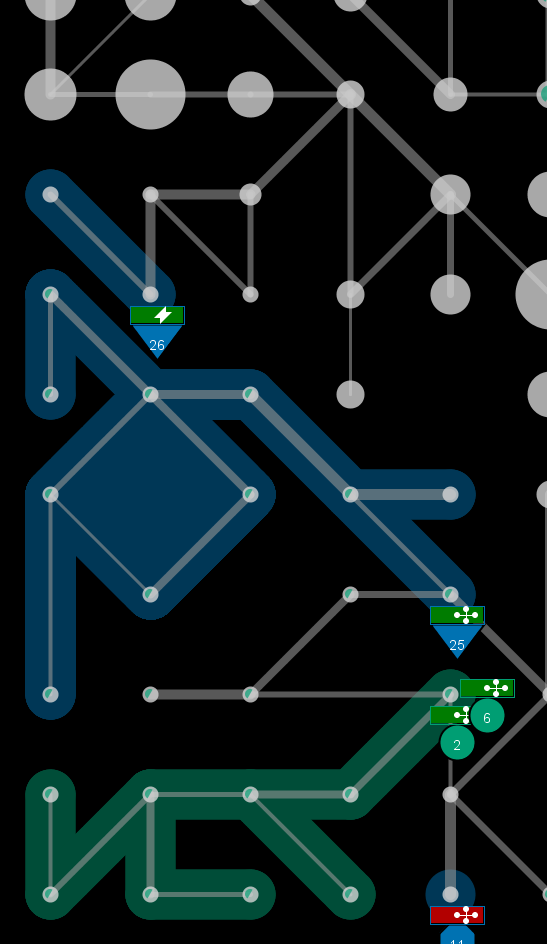
\includegraphics[height=.5\textheight]{images/articulation_points}
  \caption{By occupying an articulation point, a single agent can establish a high-scoring zone---provided that there are no enemy agents inside the subgraph that is split off from the main graph.}
  \label{fig:articulation_points}
\end{figure}
To position themselves in an optimally-scoring way, agents \emph{could} run the same algorithm locally to calculate the agent placement that will lead to the highest total sum of zone scores in each step by trying every possible permutation.
However, the number of ways to place $n$ agents on $k$ vertices is $C \left (n+r-1,r-1\right )= \frac{\left(n+r-1 \right )!}{n!\left(r-1 \right )!}$, a number that increases rapidly with $n$ and $k$.
In particular, there are $C \left (28+600-1,600-1 \right ) =\num{3.7463887025070038e+48}$ ways to place 28 agents on 600 vertices, which were the numbers used in the 2014 competition---far too many to calculate in real-time.
Finding an algorithm that calculates high-scoring zones in a limited computation time is one of the major challenges of the MAPC competition.

Our team developed a heuristic algorithm for calculating zones that will be explained below.
The goal is to find for every vertex in the graph a placement of agents around this vertex such that:
\begin{itemize}
  \item All vertices that share an edge with the centre vertex will be included in the zone.
  \item Besides the centre vertex itself, agents should only be placed on the centre vertex's two-hop neighbours.
    These are those vertices whose shortest path to the centre node has a length of two.
    Later, we will illustrate that there are rare cases in which agents must be placed on one-hop neighbours as well.
  \item The constructed zone's value per agent, that is, the sum of the values of each vertex in the zone divided by the number of agents required to establish that zone, should be high.
        Ideally, it would be maximal, but the heuristic we use does not guarantee this.
\end{itemize}
\autoref{fig:zones} shows some examples of zones that are found using our heuristic algorithm.
\begin{figure}
  \centering
  \subcaptionbox{This zone was calculated for a centre vertex that only has a degree of 1, i.e.\ that is a leaf vertex.
    Generally, it is preferable to place an agent on the articulation point that leads to a leaf vertex rather than the leaf vertex itself, as this would establish at least a zone of equal size, and possibly larger.
                 \label{fig:zones_1}}[.49\linewidth]{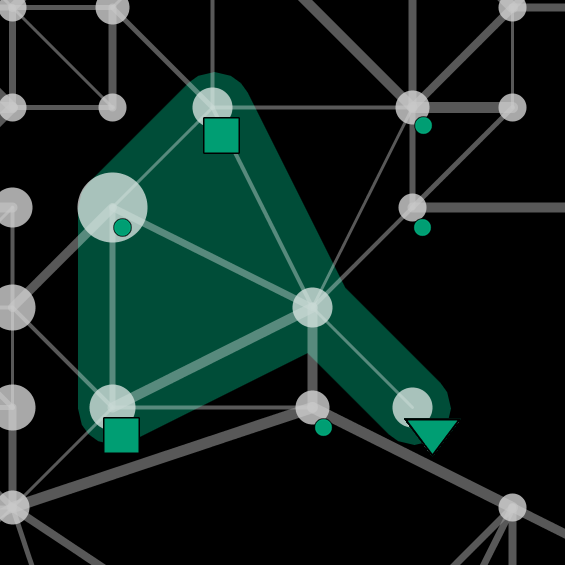
\includegraphics[width=.49\linewidth]{images/zone1.png}}
  \subcaptionbox{Here, the centre vertex has a degree of 3, and the calculated zone remains compact with only two additional agents used.
                 A lot of optional agent positions remain.
                 \label{fig:zones_2}}[.49\linewidth]{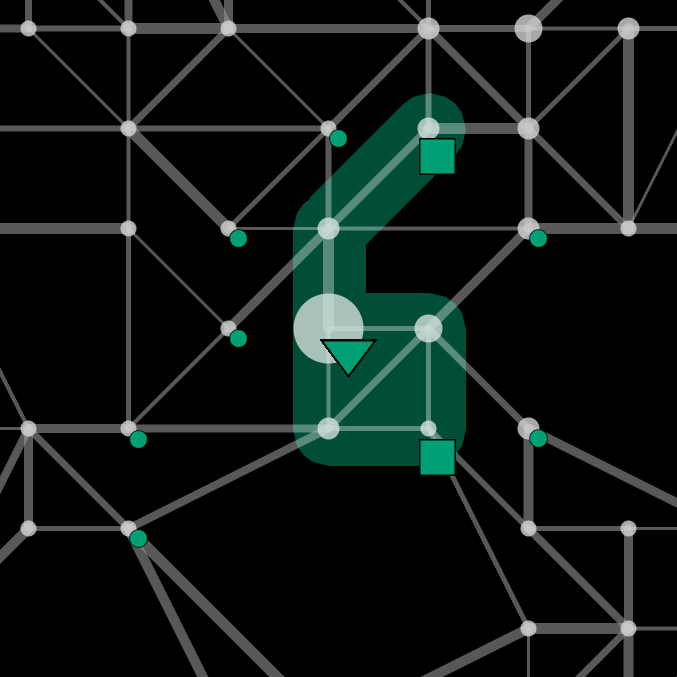
\includegraphics[width=.49\linewidth]{images/zone2.png}}
  \\
  \subcaptionbox{A zone where the centre vertex has a degree of 5, and the zone uses a total of 4 agents.
                 \label{fig:zones_3}}[.49\linewidth]{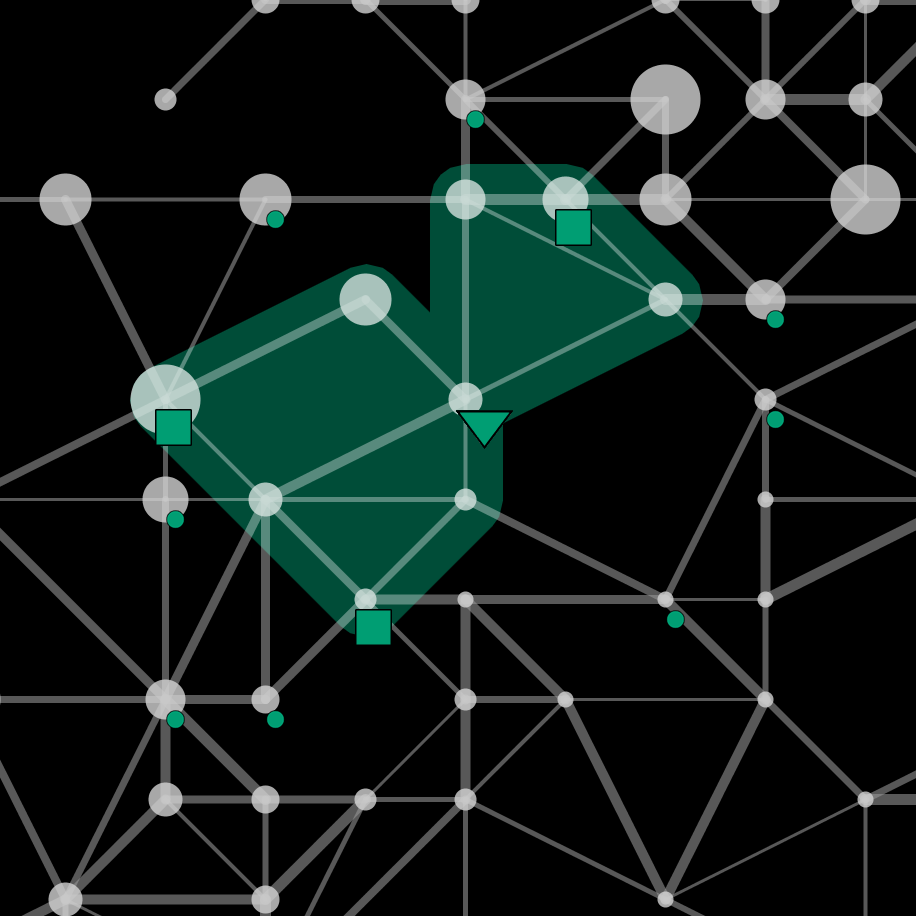
\includegraphics[width=.49\linewidth]{images/zone3.png}}
  \subcaptionbox{A zone where the centre vertex has a degree of 7, and the zone uses a total of 9 agents.
                 \label{fig:zones_4}}[.49\linewidth]{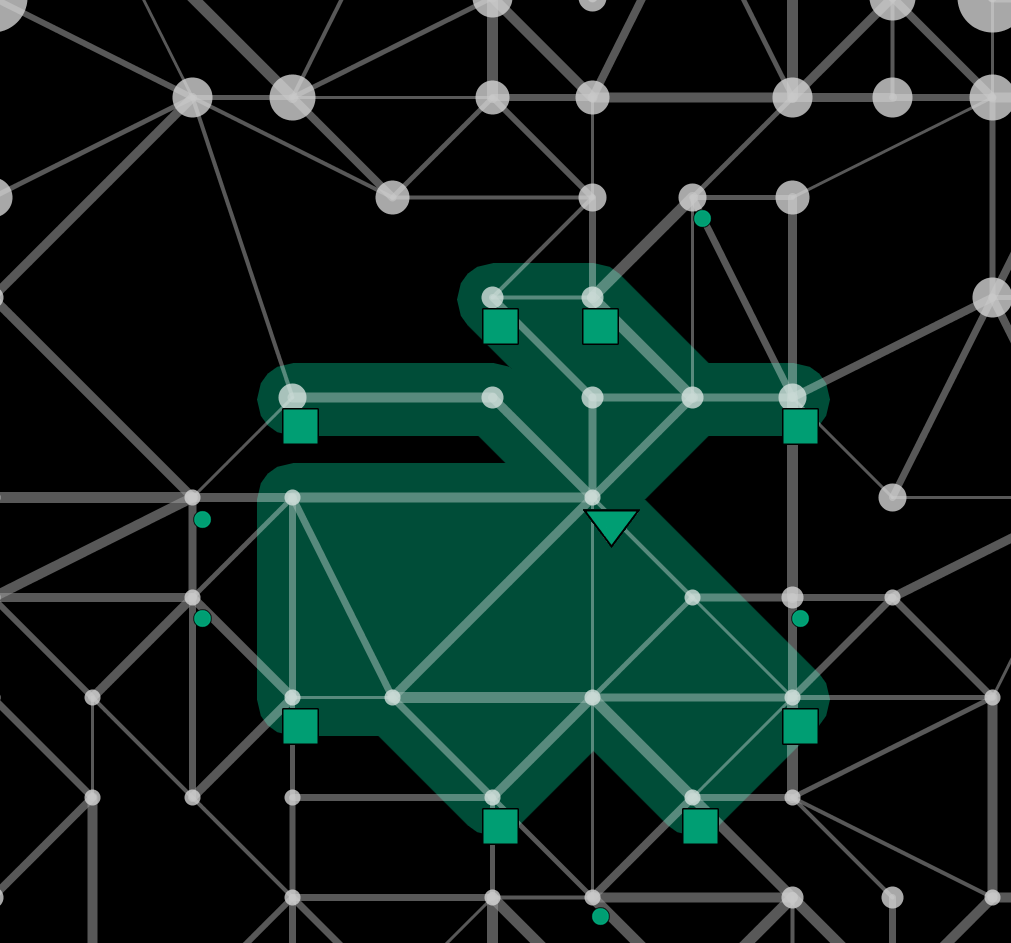
\includegraphics[width=.49\linewidth]{images/zone4.png}}
           \caption{Four examples of zones calculated by the heuristic algorithm described in \autoref{alg:zon_calculation}.
           The green squares and triangles represent the placement of agents, where the triangle is the agent on the centre vertex.
           Vertices marked with a small green circle are optional agent positions that can be used to expand the zone if there are agents left over at the end of the zone building, as described in \autoref{alg:zon_roles}.
           The green-coloured area represents the zone that is established by the given agent placement.}
  \label{fig:zones}
\end{figure}
Internally, every vertex in the graph is represented by a Java \lstinline{Vertex} object, and the calculated zone is stored as a field of that object.
The steps of the algorithm are easiest illustrated graphically, as in \autoref{fig:coloring}.
\begin{definition}
  Let $V$ be the set of vertices and $E$ the set of edges that the system knows about.
  For any $v \in V$, which we will use to denote the vertex that a zone is centred on, let $V_v^1 \subseteq V$ be the set of one-hop neighbours of $v$, that is, the set of vertices that share an edge with $v$: $V_v^1= \left\{w \middle|\left(v,w \right ) \in E\right\}$.
  Similarly, $V_v^2$ denotes the set of two-hop neighbours of $v$, i.e.\ the set of vertices that includes exactly those vertices that share an edge with any vertex in $V_v^1$, excluding those in $V_v^1$ and $v$ itself: $V_v^2= \left\{u \middle|\left(v,w \right ) \in E, \left(w,u \right ) \in E, u \notin V_v^1\cup\{v\}\right\}$.
  Let $V_v^{2+}$ denote the entire two-hop neighbourhood of $v$: $V_{v}^{2+} = \{v\} \cup V_v^1 \cup V_v^2$.
  Additionally, let $A_v$ be an initially empty set that we will use to remember vertices we want to place agents on.
  A zone and its zone value are defined as specified by the graph colouring algorithm in~\cite{ahlbrecht_mapc_2014}\todo{If we happen to explain this roughly in the MAPC section, we can further refer to that one}.
  Then, the goal of the zone calculation algorithm is to find, for every $v \in V$ in the graph, a set of agent positions $A_v \subseteq V_{v}^{2+}$ that establish a zone around $v$ so that the zone's value \emph{per agent} is high according to the heuristic used by the algorithm.
\end{definition}
Note that although $V_v^1$ and $V_v^2$ start off as defined above, by abuse of notation we will remove vertices from those sets as the algorithm progresses.
This does not mean that the structure of the graph has changed.
The algorithm for zone calculation is (re-)triggered every time a vertex in the vertex's two-hop neighbourhood $V_{v}^{2+}$ is discovered during map exploration or changes its known value.
Value changes happen when a vertex is probed by an Explorer agent.
These two events are the only ones that can lead to possible changes in $A_v$ and thus the zone.

The zone centred around vertex $v$ is is calculated through several steps:
\begin{enumerate}
  \item Initially, $A_v = \emptyset$, and $V_v^1$, $V_v^2$ and $V_v^{2+}$ as defined above.
        Iterate through every $w \in V_v^2$ and, for every $w$ that is connected directly to 2 or more vertices in $V_v^1$, add it to $A_v$ and remove it from $V_v^2$:
        \begin{multline}
        \forall w \in V_v^2: \left\{\left(w, u_1 \right ), \left(w, u_2 \right )\right\} \subseteq E, u_1 \neq u_2, \left\{u_1, u_2\right\} \subseteq V_v^1 \\
        \rightarrow A_v := A_v \cup \left\{w\right\}, V_v^2 := V_v^2 \setminus \left\{w \right \}
        \end{multline}
  \item For every $w \in V_v^2$, if $w$ is connected either directly or through a single one-hop neighbour of $v$ to any $u \in A_v$, remove it from $V_v^2$:
  \begin{multline}
  \forall w \in V_v^2: \exists u \in A_v \rightarrow V_v^2 := V_v^2 \setminus \{w\}
\\ \forall w \in V_v^2: \exists u \in A_v: \exists x \in V_v^1: \left\{\left(w, x \right ), \left(x, u \right )\right\} \subseteq E\rightarrow V_v^2 := V_v^2 \setminus \{w\}
  \end{multline}
      The reasoning behind this is that those vertices in $V_v^1$ that are neighbours of those in $A_v$ will definitely be included in the zone.
      Moreover, the vertices we remove this way will not contribute towards our goal of including all one-hop neighbours $V_v^1$ in the zone for $v$.
  \item In the next step, \enquote{bridges} are discovered in the list of remaining two-hop neighbours $V_v^2$.
        A \emph{bridge} is considered to be a connected triple of vertices where one of the vertices is directly connected to the other two.
        If such a bridge exists in $V_v^2$, all three involved vertices can be included in the zone around $v$ by placing an agent on either end of the bridge and the in-between vertex unoccupied:
        \begin{multline}
        \forall w_1, w_2, w_3 \in V_v^2: \left(w_1, w_2\right ), \left(w_2, w_3 \right ) \in E \\ \rightarrow A_v := A_v \cup \left\{w_1, w_3 \right \}, V_v^2 := V_v^2 \setminus \left\{w_1,w_2,w_3\right\}
        \end{multline}
        Since three vertices can be captured in the zone for the \enquote{cost} of two agents, we consider this a good exchange to make.
  \item Next, the algorithm checks if all one-hop neighbours $V_v^1$ are connected to the agent positions $A_v$.
        This is frequently the case, but not always.
        If a remaining, unconnected one-hop $u \in V_v^1$ is found, we check if it is directly connected to one or more of the remaining two-hop vertices in $V_v^2$.
        If that is the case, we choose the neighbouring two-hop $w \in V_v^2$ with the highest vertex value and add it to the list of agent positions $A_v$.
        If no such two-hop vertex is found, we add the unconnected one-hop vertex to the list of agent positions.
        This is the only case where a one-hop vertex can be added to the list of agent positions: \begin{multline}
        \forall w \in V_v^1: \lnot \exists u \in A_v: \left(w, u \right ) \in E \\\rightarrow \left\{\begin{array}{lcl}
A_v := A_v \cup \left\{x\right\}, V_v^2 := V_v^2 \setminus \left\{x\right\} & \textup{if} & \exists x \in V_v^2: \left(x, w \right ) \in E\\
A_v := A_v \cup \left\{w\right\} &\textup{else} &
\end{array}\right.
        \end{multline}
  \item Finally, we include the centre vertex $v$ in the list of agent positions: $A_v := A_v \cup \left\{v\right\}$.
        Any vertices that remain in $V_v^2$ are saved as additional agent positions
        They could be used to extend the zone by otherwise idle agents.
        But unlike the vertices in $A_v$ the vertices left in $V_{v}^{2}$ are not required to establish the initial smallest zone that we calculated.
\end{enumerate}
\begin{figure}
  \centering
  \subcaptionbox{Before zone calculation.
                 \label{fig:coloring1}}[.49\linewidth]{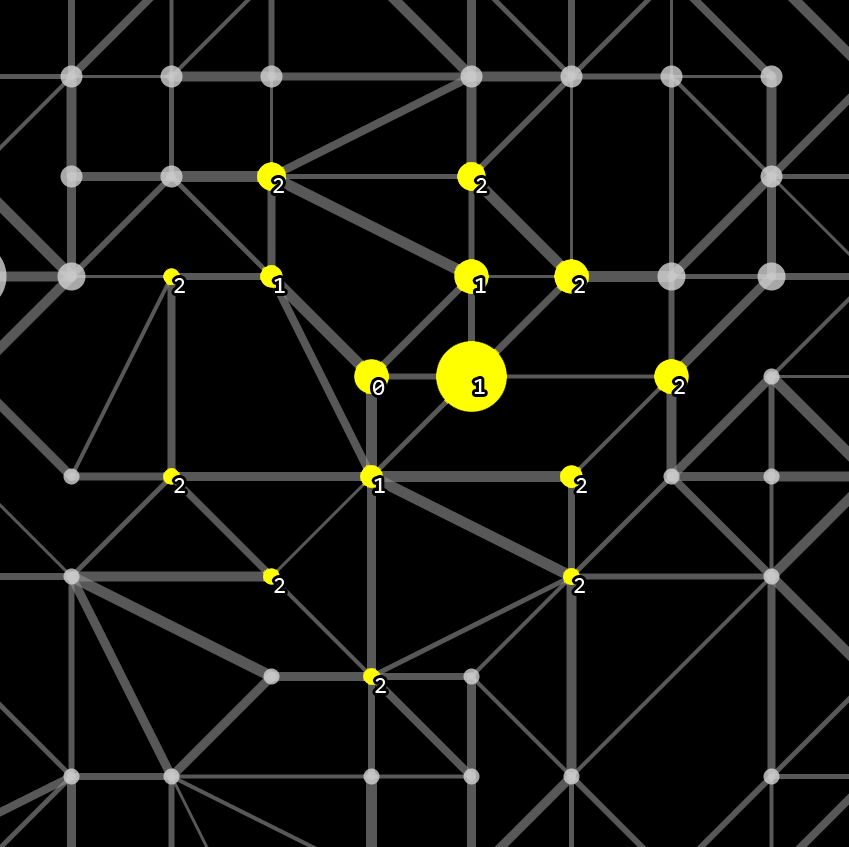
\includegraphics[width=.49\linewidth]{images/coloring1.png}}
  \subcaptionbox{After finding multiply-connected vertices in $V_v^2$ and removing their neighbouring two-hops.
                 \label{fig:coloring2}}[.49\linewidth]{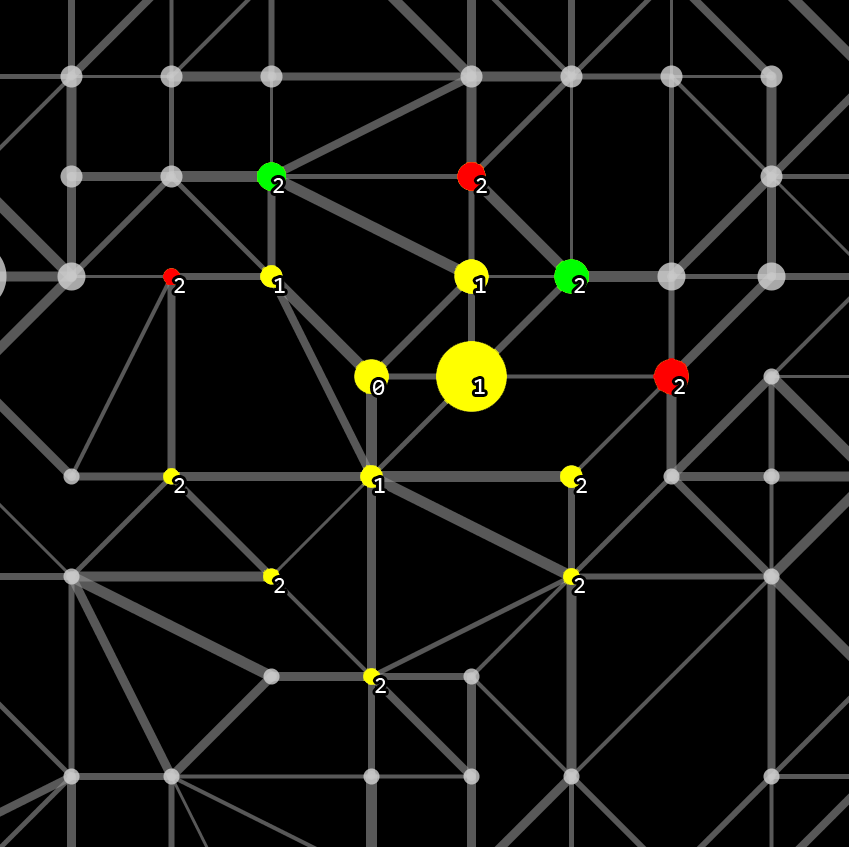
\includegraphics[width=.49\linewidth]{images/coloring2.png}}
  \\
  \subcaptionbox{Finding bridges.
                 \label{fig:coloring3}}[.49\linewidth]{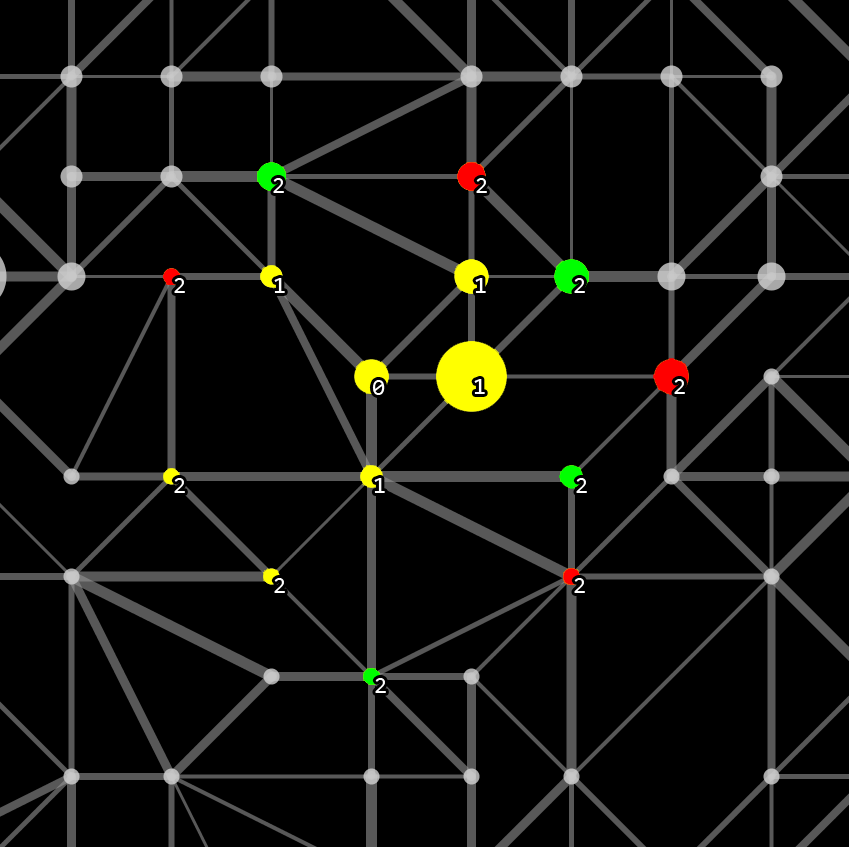
\includegraphics[width=.49\linewidth]{images/coloring3.png}}
  \subcaptionbox{After zone calculation.
                 \label{fig:coloring4}}[.49\linewidth]{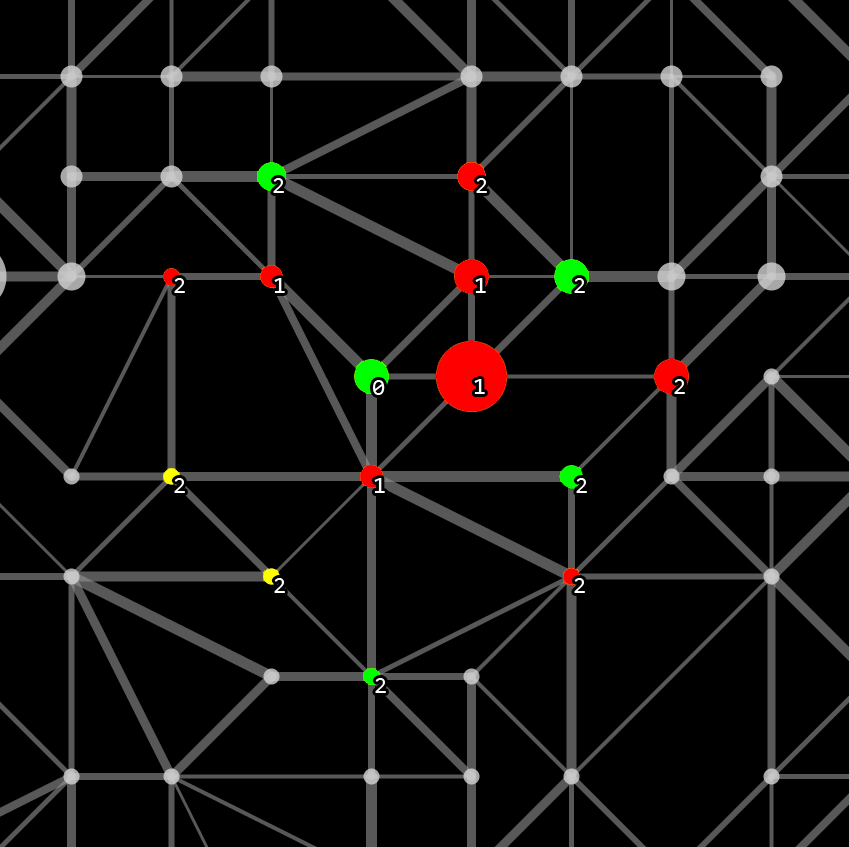
\includegraphics[width=.49\linewidth]{images/coloring4.png}}
  \caption{The zone calculation algorithm shown in four steps.
           Vertices are coloured differently according to their current state as the algorithm progresses.
           Green vertices are vertices that an agent must be placed on, so those in $A_v$.
           Red vertices are those where placing an agent would be redundant because it does not help with the goal of including all one-hop neighbours $V_v^1$ in the zone.
           Yellow vertices denote notes where agents could be placed to extend the zone, but are not considered optimal agent positions in the eyes of the algorithm.
           Numbers shown next to vertices represent their edge distance from the centre vertex $v$.}
  \label{fig:coloring}
\end{figure}
While we consider our algorithm to find zones of acceptable high zone values per agent, it can easily be shown to be suboptimal.
For one, it only considers vertices within the two-hop neighbourhood of the centre vertex
Furthermore, it is not difficult to think of possible graph structures where a different agent placement would lead to a better zone.
For example, if one of the remaining yellow vertices in \autoref{fig:coloring4} were an articulation point whose inclusion in the list of agent positions would add more than that single vertex to the zone.
Then, this would probably be a good vertex to place an agent on.
Yet, it would not be discovered by our heuristic algorithm.

\subsubsection[Zone Finding Process.]{Zone Finding Process.$^\circ$}\label{alg:zon_finding}
This section explains how agents decide on what zones should be built.
Each zone finding process can end successfully or fail for any individual agent.
If it failed, the agent is not going to be a part of a zone and a new zone finding process is started.
The first part of this section covers what changes are made so that with every failed zone finding process a successful one becomes likelier.
If a zone finding process ended succesfully, the most valuable zone known to the agents will be built.
This is ensured through agent communication which is presented in the last part of this section.
% It focusses on the communication between the agents.
Agents start looking for zones when they have finished the exploration phase.
As explained in \autoref{alg:exploration}, explorer agents do not only survey but probe as well.
Hence, other agents may finish the exploration phase earlier.
Furthermore, zones can be broken up at any time forcing the agents to start looking for a new zone again.
As a result, the zone finding process is in fact asynchronous.
Problems arising from this are mainly dealt with throughout the actual building of zones which is illustrated in \autoref{alg:zon_roles}.

In the beginning, all agents have to centrally register themselves when they are ready for zone building to indicate this availability.
Next, each agent uses the algorithm presented in \autoref{alg:zon_calculation} to determine the best zone in its neighbourhood.
The algorithm uses a range parameter $k$ which indicates the $k$-hop-neighbourhood up to which the algorithm will look for the best not yet built zone.
This range starts at $1$ and is incremented every time the agent finishes a zone finding process without being part of a zone afterwards.
As a result, it is more probable for an agent to find a zone with a high per agent score which has not been build yet.
Thus, it is also likelier for the agent to be part of a zone, because throughout every zone finding process only the most valuable zone is going to be built.
The range has a maximum to ensure that an agent will not look for zones too far away from it.
When a zone is broken up, the range will be reset, which is covered by \autoref{alg:zon_roles}.

After every agent interested in building a zone has determined the best zone in its neighbourhood, all such agents must send their best zone to all other agents.
This is because all agents ready to build a zone should know about and hence only try to build the best globally, not yet built zone.
At any time, every agent may only know about one zone.
This zone will be the best zone an agent is aware of at the moment.
Zones are being compared by their per agent score.
A higher score indicates a better zone.
Before building any zone, the agents will have to wait until the information about their best zone has reached all other agents.
This is ensured by the agent having to wait for all other agents to reply to him.
Therefore, when an agent receives information about a zone, it has two options.
One is to reply with a simple acknowledgement message expressing that it had received the message.
The other is to reply with its own zone in case that its zone is better.
Agents may not reply with information about a better zone if it is not their own.
This is to prevent duplicate messages.
Otherwise, multiple agents could reply with the same zone of which they had been informed about by the same agent.
Whenever an agent receives information about a better zone, it replaces its former knowledge about the best zone with the new one.
Agents which are not interested in building a zone but receive information about a zone simply ignore the message but reply with an acknowledgement.
This way, the sender will still be able to determine when every agent has processed the sent information.
In case the zone calculation algorithm did not return any zone to an agent, this agent has to ask all other agents for a zone.
It will accept the first reply containing zone information as its new best zone because it is better than no zone.
The agent will then continue similar to the earlier presented behaviour and wait until it received replies from all other agents.
After an agent has received all replies, it may start building a zone as illustrated in the next subsection. % TODO this only works if the order is not changed again.

\subsubsection[Zone Building Roles and the Lifecycle of a Zone.]{Zone Building Roles and the Lifecycle of a Zone.$^\circ$}\label{alg:zon_roles}
This subsection describes the two roles exclusive to zone building.
It covers the roles' associated tasks and duties throughout the lifecycle of a zone as well as the lifecycle itself.
These roles are those of a \emph{coach} and a \emph{minion}.
Each zone is built by one coach and a varying amount of minions.
Minions are agents which are dedicated to build a zone by obeying their coach's orders.
Every agent may only be part of one zone at a time.
% The last sentence is probably redundant.
The roles are assigned when the zone finding process has ended and a concrete zone is about to be built.
Agents keep either of these roles until the zone is broken up or they have to leave it.
The roles regulate the agents' behaviour throughout the time they spend in a zone.
% This subsection describes the communication hierarchy during active zoning until its breakup

Before looking at border cases, an ideal case of a zone lifecycle is presented.
There, the zone finding process described in \autoref{alg:zon_finding} ends with all agents knowing about the same best zone.
This zone was found by one agent which will then become the zone's coach.
Next, the coach informs the agents which will be part of the zone where to go to.
On receipt of this message, the agents become minions and move to their designated vertex.
The coach will also have to move to its vertex, which happens to be the centre vertex of the zone.
Furthermore, the coach will unregister itself and all its minions to indicate their unavailability to build any other zone.
In a zone, minions serve no other purpose than to occupy their designated vertex.
If a minion becomes disabled, it has to move towards a repairer agents.
Due to this, it has to leave its vertex.
Therefore, the zone can no longer exist in its original form.
In such a case, a minion has to inform its coach about its departure.
The coach must then tell all its other minions that the zone can no longer be maintained.
Consequently, all affected agents drop their role and restart looking for zones as illustrated in \autoref{alg:zon_finding}.

In reality, the zone finding process is asynchronous.
Therefore, it is likely that some agents start looking for a zone when others have nearly finished.
As a result, there can be multiple groups of agents with different knowledge about which zone would currently bring the highest score per agent.
Each group could then be expecting a different agent to become a coach.
This interferes with the assumptions that each agent may only be in one zone and have only one role at a time.
To solve this problem, coaches do not only inform their minions about where to move to.
Instead, they also transmit the per agent score of the zone they want to build together with this agent.
Any agent can then compare the received zone score with the zone it wanted to build before.
If it is higher, it must inform the coach of its former zone or its minions if it had been the coach itself.
In case that the proposed zone's score is lower than the zone the agent intended to form, it must inform the coach who just proposed the new zone.
Said coach will then have to inform all its minions that its zone is not going to be built.

Besides coaches and minions, there are also other agents who might be looking for a zone but will not be part of the one which will be built.
Such an agent will have to start a new zone finding process.
Prior to that though, it will look for any highly valuable vertex in its surrounding which is not yet occupied by anyone and move there.
The range to look for such a vertex is the same as the range for finding a zone in the agent's neighbourhood presented in \autoref{alg:zon_calculation}.
It is increased after every zone finding process which does not result in a zone where the agent is part of.
The idea is that with a wider range, the probability to find a highly valuable zone increases.
Additionally, the agent will likelier move farther away from its position in case it is not part of the zone to be built.
This should further ensure that zones are only proposed multiple times as best zones if they have a very high per agent score.

We assume due to our zone calculation algorithm that a vertex within a zone will be occupied by at most one agent.
Then, any enemy agent close to a zone endangers it.
This is because a zone may not spread across an enemy inside of it~\cite{ahlbrecht_mapc_2014}.  % p.12
Moreover, enemy saboteur agents can disable agents inside a zone, which similarly destroys the zone in its original form~\cite{ahlbrecht_mapc_2014}.  % p.11
Hence, coaches check once per step whether an enemy agent is close to the zone.
If this is the case, the coach broadcasts a message to all saboteur agents to come and defend the zone.
Saboteur agents which are not already defending a zone bid for this.
The saboteur agent closest to the zone's centre will win the bidding.
It then moves towards the enemy to disable it.
If the coach detects in a next step that the enemy moved away from the zone, it will cancel the zone defence.
The coach does so by using another broadcast as it does not know which saboteur agent was selected to defend the zone.

Explorer agents will still be probing when the first agents start looking for zones.
Therefore, the most valuable zones may change with more and more vertices being probed.
To prevent that agents build a zone once and stay there for ever if no agents attack them, zones will be split up periodically.
The periodic trigger is linked to the overall steps of the simulation and not the lifetime of each zone respectively.
Consequently, agents from different zones will have to restart looking for a zone at the same time.
In addition to allowing new zones to be build which take the information of the newly probed vertices into account, this also allows for agents to start the zone finding process in a less asynchronous fashion.
\todo{This section is missing a proper ending}

